% !TEX encoding = UTF-8 Unicode
%!TEX TS-program = xelatex

\documentclass[12pt]{extarticle}
% extarticle is like article but can handle 8pt, 9pt, 10pt, 11pt, 12pt, 14pt, 17pt, and 20pt text

\def \ititle {Origins of Mind}
 
\def \isubtitle {Lecture 08}
 
\def \iauthor {Stephen A. Butterfill}
\def \iemail{s.butterfill@warwick.ac.uk}
\date{}

%for strikethrough
\usepackage[normalem]{ulem}

\usepackage{pdfpages}


\input{$HOME/Documents/submissions/preamble_steve_handout}

%logic symbol \leftmodels
\usepackage{MnSymbol}

%\bibpunct{}{}{,}{s}{}{,}  %use superscript TICS style bib
%remove hanging indent for TICS style bib
%TODO doesnt work
\setlength{\bibhang}{0em}
%\setlength{\bibsep}{0.5em}


%itemize bullet should be dash
\renewcommand{\labelitemi}{$-$}

\begin{document}

%\raggedcolumns

\begin{multicols*}{3}

\setlength\footnotesep{1em}


\bibliographystyle{newapa} %apalike

%\maketitle
%\tableofcontents




%--------------- 
%--- start paste


\def \ititle {Logic I}
 
\def \isubtitle {Lecture 15}
 
\begin{center}
 
{\Large
 
\textbf{\ititle}: \isubtitle
 
}
 
 
 
\iemail %
 
\end{center}
 
Readings refer to sections of the course textbook, \emph{Language, Proof and Logic}.
 
 
 
\section{Soundness and Completeness: Statement of the Theorems}
 
\emph{Reading:} §8.3, §13.4
 
‘A $\vdash$ B’ means there is a proof of B using premises A
 
‘$\vdash$ B’ means there is a proof of B using no premises
 
‘A $\models$ B’ means B is a logical consequence of A
 
‘$\models$ B’ means B is a tautology
 
‘A $\models$$_{TT}$ B’ means B is a logical consequence of A just in virtue of the meanings of truth-functions (the textbook LPL calls this ‘tautological consequence’)
 
\emph{Soundness}: If A $\vdash$ B then A $\models$ B
 
\hspace{3mm} i.e. if you can prove it in Fitch, it’s valid
 
\emph{Completeness}: If A $\models$$_{TT}$ B then A $\vdash$ B
 
\hspace{3mm} i.e. if it’s valid just in virtue of the meanings of the truth-functional connectives, then you can prove it in Fitch.
 
 
 
\section{The Soundness Property and the Fubar Rules}
 
\emph{Reading:} §8.3
 
\begin{center}
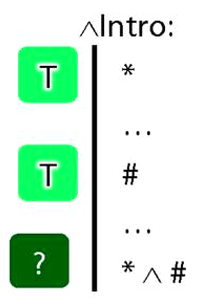
\includegraphics[scale=0.3]{img/unit_346_and.png}
\end{center}
\begin{center}
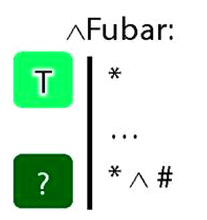
\includegraphics[scale=0.3]{img/unit_346_fubar.png}
\end{center}
 
 
\section{Proof of the Soundness Theorem}
 
\emph{Reading:} §8.3
 
\begin{minipage}{\columnwidth}
 
\textbf{Illustration of soundness proof: ∨Intro}
 
\begin{center}
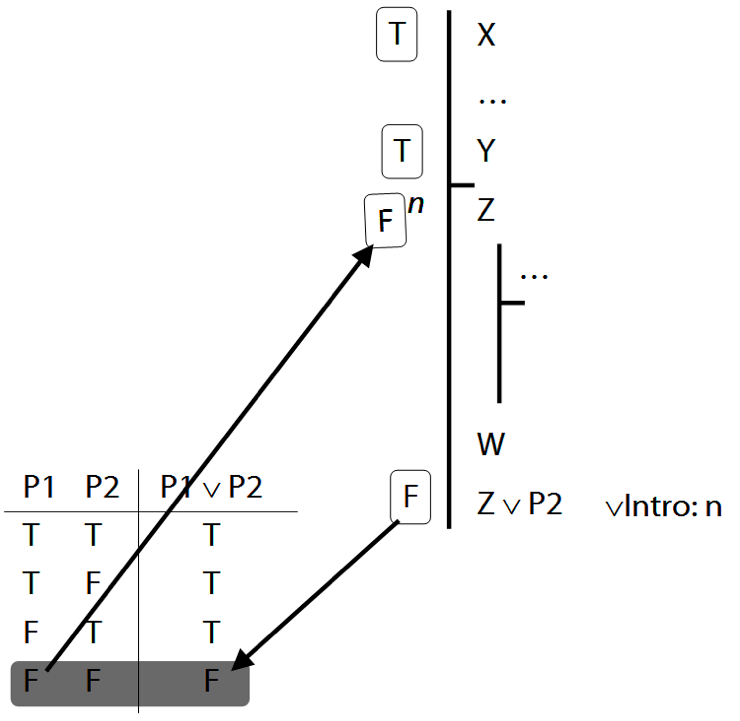
\includegraphics[scale=0.3]{img/soundness_or.png}
\end{center}
\end{minipage}
 
\emph{Useful Observation about any argument that ends with ∨Intro.} Suppose this argument is not valid, i.e. the premises are true and the conclusion false. Then Z must be false. So the argument from the premises to Z (line n) is not a valid argument. So there is a shorter proof which is not valid.
 
\emph{Stipulation}: when I say that \emph{a proof is not valid}, I mean that the last step of the proof is not a logical consequence of the premises (including premises of any open subproofs).
 
\begin{minipage}{\columnwidth}
 
\textbf{Illustration of soundness proof: ¬Intro}
 
\begin{center}
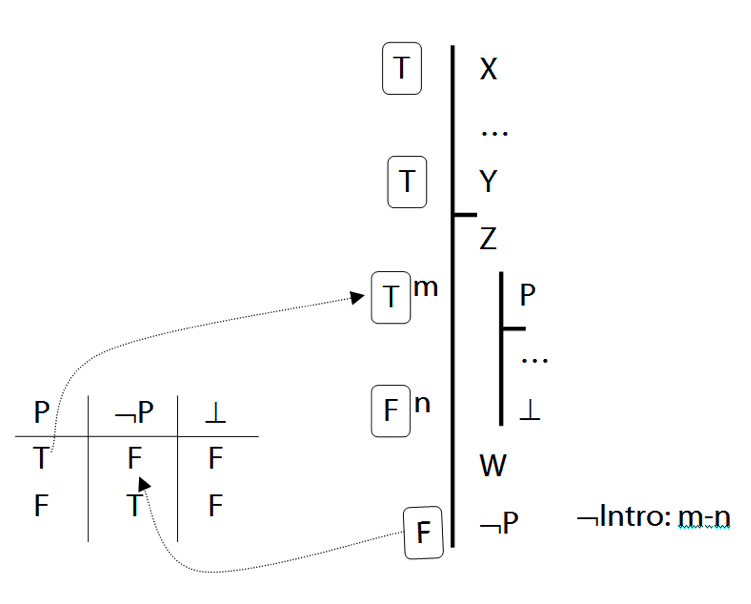
\includegraphics[scale=0.3]{img/soundness_not.png}
\end{center}
\end{minipage}
 
\begin{minipage}{\columnwidth}
 
\textbf{How to prove soundness? Outline}
 
Step 1: show that each rule has this property:
 
\hspace{5mm} Where the last step in a proof involves that rule, if proof is not valid then there is a shorter proof which is not valid.
 
Step 2: Suppose (for a contradiction) that some Fitch proofs are not valid. Select one of the shortest invalid proofs. The last step must involve one of the Fitch rules. Whichever rule it involves, we know that there must be a shorter proof which is not valid. This contradicts the fact that the selected proof is a shortest invalid proof.
 
\end{minipage}
 
 
 
\section{Translation from FOL to English}
 
Using the interpretation below, providing English translations of the following sentences of FOL.
 
\hspace{5mm} \begin{minipage}{\columnwidth}
 
\hspace{5mm} Domain: {people and actions}
 
\hspace{5mm} D(x) : x is desirable
 
\hspace{5mm} V(x) : x is virtuous
 
\hspace{5mm} A(x) : x is an action
 
\hspace{5mm} P(x,y) : x performed y
 
\hspace{5mm} a : Ayesha
 
\end{minipage}
 
i. ∀x( D(x) → V(x) )
 
ii. ∀x( (A(x) ∧ D(x)) → V(x) )
 
iii. ∃x( A(x) ∧ ¬D(x) )
 
iv. ∃x( A(x) ∧ ¬D(x) ∧ V(x) )
 
v. ∃x( A(x) ∧ P(a,x) ∧ ¬V(x) )
 
vi. ¬∃x(
 
\hspace{5mm} ∃y( A(y) ∧ P(x,y) ∧ ¬V(y) )
 
\hspace{5mm} ∧
 
\hspace{5mm} ¬∃z( A(z) ∧ P(x,z) ∧ V(z) )
 
)
 
 
 
\section{Numerical Quantifiers}
 
\emph{Reading:} §14.1
 
There are at least two squares:
 
\hspace{5mm} ∃x ∃y ( Square(x) ∧ Square(y) ∧ ¬x=y )
 
At least two squares are broken:
 
\hspace{5mm} ∃x ∃y (
 
\hspace{10mm} Square(x) ∧ Broken(x)
 
\hspace{10mm} ∧
 
\hspace{10mm} Square(y) ∧ Broken(y)
 
\hspace{10mm} ∧
 
\hspace{10mm} ¬x=y
 
\hspace{5mm} )
 
There are at least three squares:
 
\hspace{5mm} ∃x ∃y ∃z (
 
\hspace{10mm} Square(x) ∧ Square(y) ∧ Square(z)
 
\hspace{10mm} ∧
 
\hspace{10mm} ¬x=y ∧ ¬y=z ∧ ¬x=z
 
\hspace{5mm} )
 
There are at most two squares:
 
\hspace{5mm} ¬There are at least three squares
 
\hspace{5mm} ¬∃x ∃y ∃z ( Square(x) ∧ Square(y) ∧ Square(z) ∧ ¬x=y ∧ ¬y=z ∧ ¬x=z)
 
There are exactly two squares:
 
\hspace{5mm} There are at most two squares ∧ There are at least two squares
 
\textbf{Number: alternatives}
 
There is at most one square:
 
\hspace{5mm} ∀x ∀y ( (Square(x) ∧ Square(y)) → x=y )
 
There are at most two squares:
 
\hspace{5mm} ∀x ∀y ∀z (
 
\hspace{10mm} (Square(x) ∧ Square(y) ∧ Square(z))
 
\hspace{10mm} →
 
\hspace{10mm} (x=y ∨ y=z ∨ x=z)
 
\hspace{5mm} )
 
There is exactly one square:
 
\hspace{5mm} ∃x ( Square(x) ∧ ∀y( Square(y) → x=y ) )
 
There are exactly two squares:
 
\hspace{5mm} ∃x∃y (
 
\hspace{10mm} Square(x) ∧ Square(y) ∧ ¬x=y
 
\hspace{10mm} ∧
 
\hspace{10mm} ∀z( Square(z) → (z=x ∨ z=y) )
 
\hspace{5mm} )
 
 
 
\section{There Is Exactly One}
 
There is one creator (at least one, maybe more).
 
\hspace{3mm} ∃x Creator(x)
 
Brian is the one and only creator.
 
\hspace{3mm} Creator(b) ∧ ∀x( Creator(x) → x=b )
 
All squares are broken.
 
\hspace{3mm} ∀x( Sqr(x) → Brkn(x) )
 
There is one and only one creator.
 
\hspace{3mm} ∃y( Creator(y) ∧ ∀x( Creator(x) → x=y ) )
 
\hspace{3mm} or:
 
\hspace{3mm} ∃y ∀x( Creator(x) ↔ x=y )
 
\section{Extra Exercises: Proofs}
 
You may not have time to do these exercises involving proofs until after term, but it would be a good idea to complete them at some point.
 
\hspace{5mm} 13.6, 13.7, *13.8, *13.9
 
\hspace{5mm} 13.19, 13.23--13.27, *13.28--13.31
 
\hspace{5mm} *13.33, 13.35, 13.37, 13.39
 
\hspace{5mm} 13.43--13.45, 13.49--13.50, *13.51--13.52
 
\vfill
\begin{minipage}{\columnwidth}
\section{Exercises}
These exercises will be discussed in seminars the week after this lecture.
The numbers below refer to the numbered exercises in the course textbook, e.g.\ `1.1' refers to exercise 1.1. on page 39 of the second edition of \emph{Language, Proof and Logic}. Exercises marked `*' are optional.
 
\begin{quote}
7.32
 
14.1--14.3, (*14.4--14.5)
 
14.10--14.12, *14.13
 
\end{quote}
\end{minipage}


%--- end paste
%--------------- 
 


\end{multicols*}

\end{document}